\documentclass[dvipsnames, tikz]{standalone}




\begin{document}
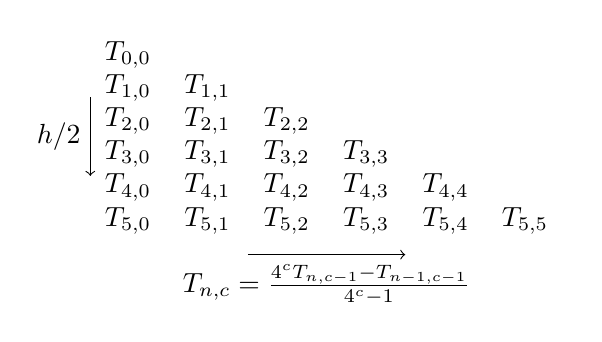
\begin{tikzpicture}
\node (A) at (0,0) {
\begin{tabular}{cccccc}
$T_{0,0}$\\
$T_{1,0}$ & $T_{1,1}$\\
$T_{2,0}$ & $T_{2,1}$ & $T_{2,2}$\\
$T_{3,0}$ & $T_{3,1}$ & $T_{3,2}$ & $T_{3,3}$\\
$T_{4,0}$ & $T_{4,1}$ & $T_{4,2}$ & $T_{4,3}$ & $T_{4,4}$\\
$T_{5,0}$ & $T_{5,1}$ & $T_{5,2}$ & $T_{5,3}$ & $T_{5,4}$ & $T_{5,5}$
\end{tabular}};

\draw[->] (-1,-1.5) -- (1,-1.5) node[anchor=north,midway] {$T_{n,c}=\frac{4^cT_{n,c-1}-T_{n-1,c-1}}{4^c-1}$};

\draw[->] (-3,0.5) -- (-3,-0.5) node[anchor=east,midway] {$h/2$};

\end{tikzpicture}
\end{document}